% !TeX root = ..\..\notes-main.tex
\documentclass[../notes-main.tex]{subfiles}
\begin{document}
\section{Topic 3: Concept of Complex Frequency}
Complex frequency is found commonly in electrical engineering. It is often notated as \( j\omega \) or \( s = \sigma \pm j \omega \). These frequencies always come in pairs, so the use of \( \pm \) is implicit to this, as complex numbers have complex conjugates, i.e.
\(s = \sigma + j \omega \) has the conjugate \(s = \sigma - j\omega \).
\begin{figure}[H]
    \centering
    \tikzsetnextfilename{complex_plane_diagram} 
    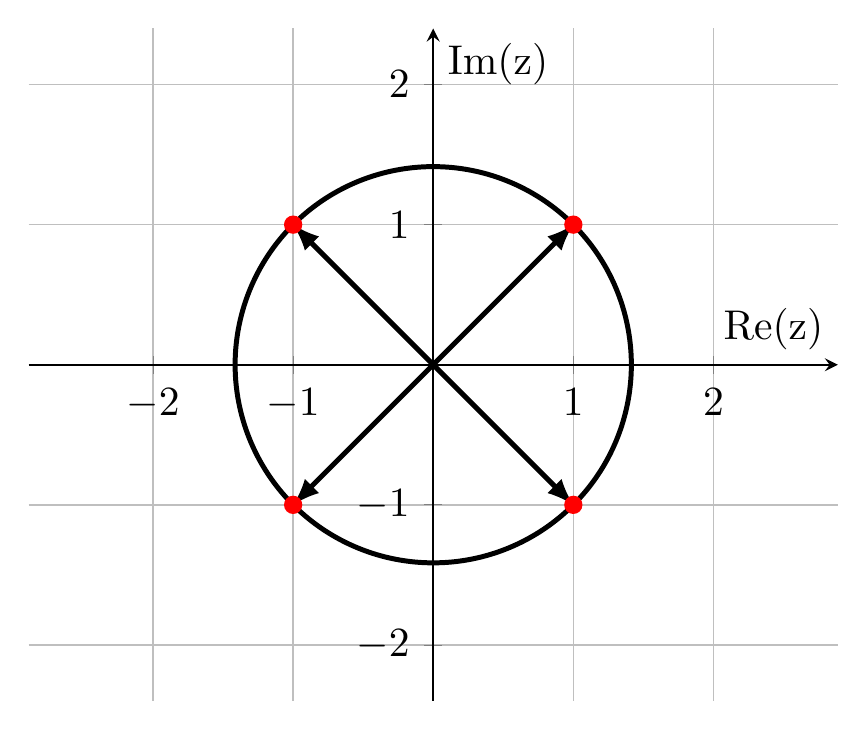
\begin{tikzpicture}[scale=1.5]
        \begin{axis}[
                axis equal,
                axis x line = middle,
                axis y line = middle,
                xmin=-2, xmax=2,
                ymin=-2, ymax=2,
                xlabel={Re(z)},
                ylabel={Im(z)},
                grid=major,
                enlargelimits=true,
            ]
            % Plot the circle |z| = sqrt(2)
            \addplot[domain=0:360, samples=200, smooth, very thick]({sqrt(2)*cos(x)}, {sqrt(2)*sin(x)});
            \addplot[only marks, mark=*, red, mark size=2pt] coordinates {%
                    (1,1) (-1,1) (1,-1) (-1,-1)
                };
            \addplot[->, black, very thick, >= latex] coordinates {(0,0) (1,1)};
            \addplot[->, black, very thick, >= latex] coordinates {(0,0) (-1,1)};
            \addplot[->, black, very thick, >= latex] coordinates {(0,0) (1,-1)};
            \addplot[->, black, very thick, >= latex] coordinates {(0,0) (-1,-1)};
        \end{axis}
    \end{tikzpicture}
    \caption{Plot of the circle \(|z| = \sqrt{2}\)}\label{fig:pgfplots-complex-plane-diagram}
\end{figure}
\noindent This is also backed up by De Moivre's Formula, which is defined mathematically as:
\begin{gather}
    \forall x \in \mathbb{R}, \quad \forall n \in \mathbb{Z}, \\
    \expfn{-jn}{x} = \cos(n x) + j \sin(n x)
    \label{eq:de-moivre-formula}
\end{gather}
Or more generally for our applications:
\begin{gather}
    \expfn{j}{x} = \cos(x) + j\sin(x) \\
    \text{Where} \, x \in \mathbb{R}\, \text{(\(x\) is Real)} \\
    \text{and} \, j \equiv i = \sqrt{-1}.
    \label{eq:de-moivre-formula-general}
\end{gather}
\noindent This means that:
\begin{mdframed}
    \begin{center}
        \redtext{\emph{A complex frequency \(j\omega \) represents a pure sinusoidal signal of frequency \(\omega \) \unit{\rads}}}
    \end{center}
\end{mdframed}\label{fig:complex-sinusoid-def-1}
\noindent For example, if a signal has a complex frequency  \compfreq{314}, then this corresponds to a pure sinusoid of frequency \freq{314} (i.e. \SI{50}{\hertz}).\\ 
Furthermore:
\begin{mdframed}
    \begin{center}
        \redtext{%
            \emph{A complex frequency \(s = \sigma + j\omega \) represents an exponentially
                damped signal of frequency \(\omega \) \unit{\rads}, and decays/amplifies at a rate decided by \(\sigma \).}}
    \end{center}
\end{mdframed}\label{fig:exp-sinusoid-def-sigma}
\noindent For example, the signal \(f(t) = \expfn{-10}{t}\sin(40\pi t) \) would look like this:
\begin{figure}[H]
    \centering
    \tikzsetnextfilename{exp_damped_sinusoid_plot}
    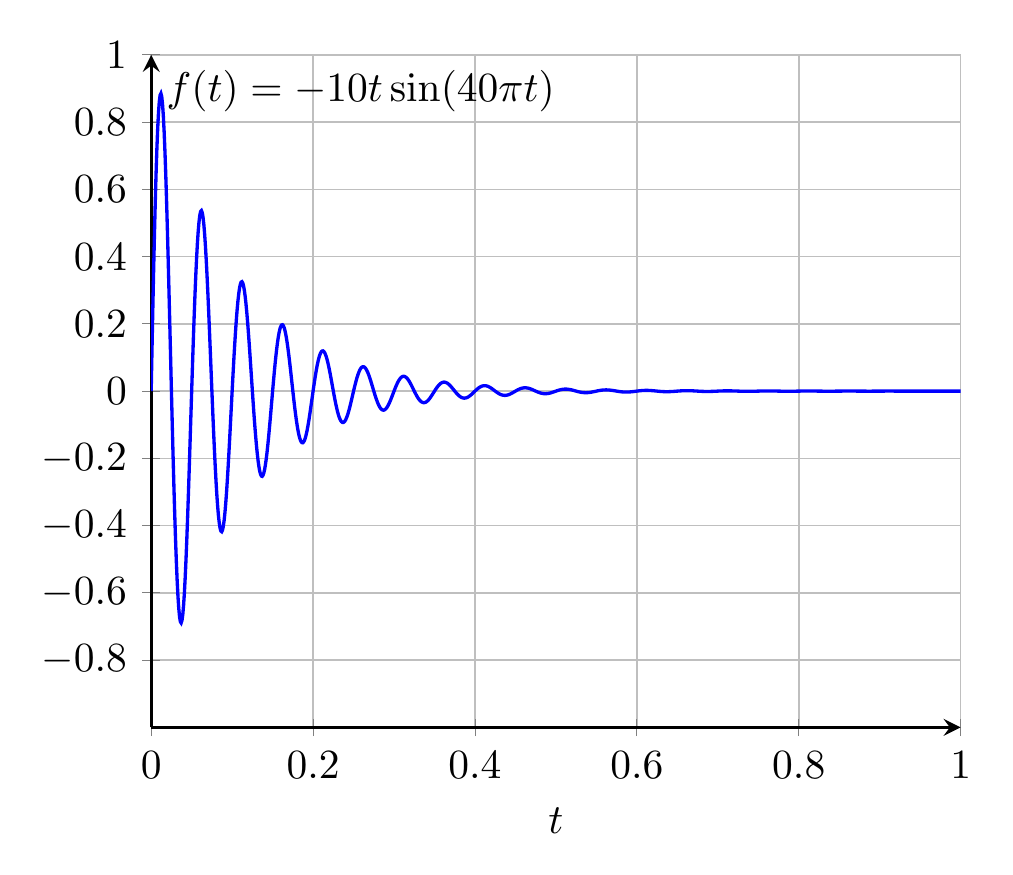
\begin{tikzpicture}[scale=1.5]
        \begin{axis}[
                domain=0:1, 
                samples=1000,
                xlabel={\(t\)},
                ylabel={\(f(t) = \expfn{-10}{t} \sin(40\pi t)\)},
                grid=major,
                thick,
                enlargelimits=true,
                axis y line = center,
                axis x line = left,
                ymin=-1, ymax=1,
                xmin=0, xmax=1,
                ytick={-1,-0.8,-0.6,-0.4,-0.2,0,0.2,0.4,0.6,0.8,1},
            ]
            \addplot[blue, thick] {exp(-10*x) * sin(deg(40*pi*x))};
        \end{axis}
    \end{tikzpicture}\caption{Plot of the signal \(f(t) = \expfn{-10}{t}\sin(40\pi t)\).}\label{fig:exp-damped-sinusoid-plot-pgf}
\end{figure}
\end{document}